%==========================================
%
% SIBGRAPI 2026 paper template
% Example of IEEEtran.cls
%
%==========================================

% *** Authors should verify (and, if needed, correct) their LaTeX system  ***
% *** with the testflow diagnostic prior to trusting their LaTeX platform ***
% *** with production work. The IEEE's font choices and paper sizes can   ***
% *** trigger bugs that do not appear when using other class files.       ***                          ***
% The testflow support page is at:
% http://www.michaelshell.org/tex/testflow/

\documentclass[10pt,conference]{IEEEtran}


% Some very useful LaTeX packages include:
% (uncomment the ones you want to load)



% *** MISC UTILITY PACKAGES ***
%
%\usepackage{ifpdf}
% Heiko Oberdiek's ifpdf.sty is very useful if you need conditional
% compilation based on whether the output is pdf or dvi.
% usage:
% \ifpdf
%   % pdf code
% \else
%   % dvi code
% \fi
% The latest version of ifpdf.sty can be obtained from:
% http://www.ctan.org/pkg/ifpdf
% Also, note that IEEEtran.cls V1.7 and later provides a builtin
% \ifCLASSINFOpdf conditional that works the same way.
% When switching from latex to pdflatex and vice-versa, the compiler may
% have to be run twice to clear warning/error messages.

\usepackage{subcaption}
\usepackage{xcolor}
\usepackage{tikz}
\usepackage{fontawesome5}
\usepackage{float}
\usepackage{booktabs}
\usepackage{multirow}
\usepackage{amssymb}
\usetikzlibrary{positioning, fit, arrows.meta, backgrounds}

% *** CITATION PACKAGES ***
%
\usepackage{cite}
% cite.sty was written by Donald Arseneau
% V1.6 and later of IEEEtran pre-defines the format of the cite.sty package
% \cite{} output to follow that of the IEEE. Loading the cite package will
% result in citation numbers being automatically sorted and properly
% "compressed/ranged". e.g., [1], [9], [2], [7], [5], [6] without using
% cite.sty will become [1], [2], [5]--[7], [9] using cite.sty. cite.sty's
% \cite will automatically add leading space, if needed. Use cite.sty's
% noadjust option (cite.sty V3.8 and later) if you want to turn this off
% such as if a citation ever needs to be enclosed in parenthesis.
% cite.sty is already installed on most LaTeX systems. Be sure and use
% version 5.0 (2009-03-20) and later if using hyperref.sty.
% The latest version can be obtained at:
% http://www.ctan.org/pkg/cite
% The documentation is contained in the cite.sty file itself.


% *** GRAPHICS RELATED PACKAGES ***
%
\ifCLASSINFOpdf
   \usepackage{graphicx}
  % declare the path(s) where your graphic files are
   \graphicspath{{img/}}
  % and their extensions so you won't have to specify these with
  % every instance of \includegraphics
   \DeclareGraphicsExtensions{.pdf,.jpeg,.png}
\else
  % or other class option (dvipsone, dvipdf, if not using dvips). graphicx
  % will default to the driver specified in the system graphics.cfg if no
  % driver is specified.
   \usepackage[dvips]{graphicx}
  % declare the path(s) where your graphic files are
   \graphicspath{{../img/}}
  % and their extensions so you won't have to specify these with
  % every instance of \includegraphics
   \DeclareGraphicsExtensions{.eps}
\fi

% *** MATH PACKAGES ***
%
\usepackage[cmex10]{amsmath}
% A popular package from the American Mathematical Society that provides
% many useful and powerful commands for dealing with mathematics.
%
% Note that the amsmath package sets \interdisplaylinepenalty to 10000
% thus preventing page breaks from occurring within multiline equations. Use:
\interdisplaylinepenalty=2500
% after loading amsmath to restore such page breaks as IEEEtran.cls normally
% does. amsmath.sty is already installed on most LaTeX systems. The latest
% version and documentation can be obtained at:
% http://www.ctan.org/pkg/amsmath
\usepackage{amsthm}
\newtheorem{definition}{Definition}

% *** SPECIALIZED LIST PACKAGES ***
%
\usepackage{algorithmic}

% *** ALIGNMENT PACKAGES ***
%
\usepackage{array}
% *** SUBFIGURE PACKAGES ***
\ifCLASSOPTIONcompsoc
  \usepackage[caption=false,font=normalsize,labelfont=sf,textfont=sf]{subfig}
\else
  \usepackage[caption=false,font=footnotesize]{subfig}
\fi

\usepackage{stfloats}

% *** PDF, URL AND HYPERLINK PACKAGES ***
%
\usepackage{url}

% correct bad hyphenation here
\hyphenation{op-tical net-works semi-conduc-tor}

%------------------------------------------------------------------------- 
% change the % on next lines to produce the final camera-ready version 
\newif\iffinal
\finalfalse
%\finaltrue
\newcommand{\cmtid}{99999}
%------------------------------------------------------------------------- 

\iffinal
\else
\usepackage[switch]{lineno}
\fi

\begin{document}
\title{Generalizable and Per-Scene NeRF Architectures under Sparse-View Conditions: A Systematic Benchmarking Methodology}

% author names and affiliations
% use a multiple column layout for up to two different
% affiliations


% for over three affiliations, or if they all won't fit within the width
% of the page, use this alternative format: 
%\author{\IEEEauthorblockN{
%Felipe Gomes da Silva\IEEEauthorrefmark{1},
%Leandro A. Neves\IEEEauthorrefmark{1},
%Guilherme F. Roberto\IEEEauthorrefmark{1},
%Oliveira\IEEEauthorrefmark{2}\textsuperscript{,}\IEEEauthorrefmark{3},\\
%Adriano B. Silva\IEEEauthorrefmark{3}, 
%Tha\'ina A. A. Tosta\IEEEauthorrefmark{4},
%Marcelo Z. do Nascimento\IEEEauthorrefmark{3} and
%Thiago Pozati\IEEEauthorrefmark{1}}

%\IEEEauthorblockA{\IEEEauthorrefmark{1}Department of Computer Science and Statistics (DCCE)\\ São Paulo State University (UNESP), São José do Rio Preto, SP, Brazil\\ Email: felipe.gomes-silva@unesp.br, leandro.neves@unesp.br}

%\IEEEauthorblockA{\IEEEauthorrefmark{2}Federal Institute of Education, Science and Technology of São Paulo (IFSP)\\ São Paulo, SP, Brazil\\ Email: domingos.oliveira@ifsp.edu.br}

%\IEEEauthorblockA{\IEEEauthorrefmark{3}Faculty of Computer Science (FACOM)\\ Federal University of Uberlândia (UFU), Uberlândia, MG, Brazil\\ Email: adriano.barbosa@ufu.br, marcelo.nascimento@ufu.br}

%\IEEEauthorblockA{\IEEEauthorrefmark{4}Department of Computing and Mathematics\\ University of São Paulo (USP), Ribeirão Preto, SP, Brazil\\ Email: tosta.thaina@usp.br}
%}




% make the title area
\maketitle

\begin{abstract}
This work proposes a methodology for systematically evaluating the trade-offs between computational performance and reconstruction fidelity of Neural Radiance Field (NeRF) architectures under sparse-view conditions. Four representative methods are evaluated using visual fidelity metrics, including Peak Signal-to-Noise Ratio (PSNR), Structural Similarity Index Measure (SSIM), and Learned Perceptual Image Patch Similarity (LPIPS), together with computational performance metrics, including training convergence time, Video Random Access Memory (VRAM) footprint, and inference latency. The experimental results reveal a clear trade-off between reconstruction fidelity and computational efficiency. Per-Scene models consistently outperform Generalizable models in visual quality, achieving up to 27.11 dB PSNR, 0.875 SSIM, and 0.171 LPIPS, while also providing significantly higher inference throughput and lower memory consumption. In contrast, generalizable models offer greater flexibility for acquisition-constrained scenarios but exhibit limited reconstruction fidelity and unstable optimization under severe sparse-view conditions. The proposed methodology and the resulting quantitative analyses establish a standardized and reproducible framework for benchmarking heterogeneous neural rendering architectures, enabling systematic model selection according to computational and acquisition constraints.
\end{abstract}

% For peerreview papers, this IEEEtran command inserts a page break and
% creates the second title. It will be ignored for other modes.
\IEEEpeerreviewmaketitle


\section{Introduction}
\label{sec:intro}

Neural Radiance Fields (NeRFs) have consolidated themselves in recent years as the state-of-the-art for novel view synthesis, in both industry and academia \cite{kerbl3Dgaussians, Tancik2023, substance3dviewer}. However, the most advanced neural rendering techniques require considerable computational resources and multi-view datasets for training. Both challenges make practical applications, such as mobile scanning, virtual try-ons, and synthesis in reduced datasets, unfeasible.To address this problem, several methods have been proposed to advance the state of the art, including Instant-NGP (\textit{Instant Neural Graphics Primitives}), Nerfacto, PixelNeRF, and GNT (\textit{Generalizable NeRF Transformer}) \cite{muller2022, Tancik2023, yu2021pixelnerfneuralradiancefields, t2023attentionnerfneeds}. These methods investigate different aspects of neural rendering, such as spatial \textit{encoding} \cite{muller2022}, hybrid architectures that combine Convolutional Neural Networks (CNNs) and Vision Transformers (ViTs) \cite{schwarz2021grafgenerativeradiancefields, wu2021cvt, t2023attentionnerfneeds}, and model pre-computation (\textit{baking}) into compact representations with a reduced memory footprint \cite{hedman2021bakingneuralradiancefields}.

In this context, this work investigates the application of different NeRF models and their respective optimization techniques to sparse-view datasets by developing a methodology for evaluating the trade-off between computational performance and the visual quality of the reconstructed volumes. Reconstruction fidelity was assessed using three widely adopted image quality metrics: PSNR (\textit{Peak Signal-to-Noise Ratio}), SSIM (\textit{Structural Similarity Index Measure}) \cite{wang2004image}, and LPIPS (\textit{Learned Perceptual Image Patch Similarity}) \cite{zhang2018unreasonable}. The operational cost of each model was quantified using system-level performance metrics, including training convergence time, inference speed, and memory footprint, particularly VRAM (\textit{Video Random Access Memory}) consumption. Although previous studies have investigated NeRFs under limited-data settings \cite{niemeyer2022regnerf, kim2023poserefinement}, and benchmarking frameworks such as NerfBaselines \cite{kulhanek2025nerfbaselinesconsistentreproducibleevaluation} have evaluated traditional and per-scene NeRF models, a systematic comparison of generalizable neural rendering architectures employing convolutional and attention-based feature extractors under controlled hardware conditions and reproducible data splits remains absent from the literature. To bridge this gap, this work develops a systematic evaluation methodology for quantitatively assessing the trade-offs between computational efficiency and reconstruction fidelity across four neural rendering architectures under three sparse-view data regimes. Thus, the main contributions of this work are: (i) the formulation of a unified evaluation protocol for few-shot and per-scene NeRF architectures, ensuring reproducibility through standardized data partitions, controlled execution environments, and consistent evaluation metrics across three sparse-view data regimes; and (ii) the implementation and public release of integration wrappers that extend the Nerfstudio framework with PixelNeRF and GNT, providing a common experimental infrastructure for standardized benchmarking of heterogeneous neural rendering architectures.


\section{Theoretical Background}
\label{sec:fund}

\subsection{Neural Radiance Fields and Volumetric Rendering}
The foundational architecture of NeRFs utilizes Multilayer Perceptrons (MLPs) to approximate a continuous 5D scene representation \cite{mildenhall2020nerfrepresentingscenesneural}. This function takes a spatial position $\mathbf{x} = (x, y, z)$ and a viewing direction $\mathbf{d} = (\theta, \phi)$ as inputs, outputting the volumetric density $\sigma(\mathbf{x})$ and associated color $\mathbf{c} = (r, g, b)$:

$$
\gamma(\mathbf{x}, \mathbf{d}) \rightarrow \mathbf{v}, \quad F_\theta'(\mathbf{v}) \rightarrow (\sigma, \mathbf{c}), \quad \sigma \in \mathbb{R}_{\geq 0},\ \mathbf{c} \in [0, 1]^3
$$
where $\theta$ represents the neural network weights, $F_\theta'$ is the original MLP, and $\gamma$ is a positional encoder mapping inputs into a higher-dimensional feature vector $\mathbf{v}$.

To synthesize novel views, the expected color of a pixel is computed via volumetric rendering. For a ray $\mathbf{r}(t) = \mathbf{o} + t\mathbf{d}$ with depth bounds $(t_n, t_f)$, the resulting color is:
$$\hat{C}(\mathbf{r}) = \int_{t_n}^{t_f} T(t) \sigma(\mathbf{r}(t)) \mathbf{c}(\mathbf{r}(t), \mathbf{d}) \, dt$$
where $T(t) = \exp\left(-\int_{t_n}^t \sigma(\mathbf{r}(s)) \, ds\right)$ denotes the accumulated transmittance. In practice, this integral is numerically approximated via alpha compositing over discrete samples along each ray.

\subsection{Architectural Optimizations and Generalization}
Although the original NeRF achieves high-fidelity results, its reliance on large MLPs imposes computational bottlenecks. To accelerate optimization, hybrid representations were introduced to replace Fourier positional encoding with hash encoding. Instant-NGP proposes a multiscale hash table that maps spatial coordinates to feature vectors, heavily reducing optimization time \cite{muller2022}. Nerfacto builds upon this mechanism by combining multiresolution hash encoding with proposal sampling, pose refinement, spherical harmonics, and appearance embeddings to balance visual quality and rendering speed \cite{Tancik2023}.

These per-scene methods, however, fundamentally rely on dense multi-view observations. In practical scenarios, such as mobile scanning, virtual try-on, and medical imaging (for instance, histology and holotomography), multi-view acquisition is often physically limited \cite{ijms24076747}. Under these sparse-view constraints, lacking camera pose redundancy, per-scene models suffer geometric degradation.

To synthesize novel views from sparse inputs, few-shot generalizable NeRFs incorporate structural priors learned from large datasets via dedicated feature extractors. PixelNeRF  applies a pre-trained Residual ResNet to extract spatial features from 2D projections, conditioning the radiance MLP \cite{yu2021pixelnerfneuralradiancefields}. GNT replaces the CNN with a vision transformer for global feature extraction, and substitutes the MLP with a cross-attention transformer to aggregate multi-view information \cite{t2023attentionnerfneeds}.

To maximize visual fidelity, generalizable models frequently employ fine-tuning (FT). Instead of purely zero-shot (ZS) inference, FT updates the network weights using the sparse views of the novel scene as direct photometric supervision. This rapid optimization reduces the domain gap, though it carries the risk of representational collapse if overfitted.


Given the fundamental architectural differences between per-scene optimizations and generalizable priors, selecting the optimal model for sparse-view deployments remains non-trivial. Consequently, a standardized evaluation framework is essential to systematically benchmark these trade-offs, which forms the core methodology of this work.

\section{Materials and Methods}
\label{sec:methods}

\begin{figure}[!t]
\centering
% Color definitions
\definecolor{mainborder}{rgb}{0.18, 0.24, 0.35}     % Sleek steel navy
\definecolor{mainfill}{rgb}{0.94, 0.95, 0.97}       % Elegant light slate gray
\definecolor{secborder}{rgb}{0.35, 0.43, 0.53}     % Soft slate/steel blue
\definecolor{secfill}{rgb}{0.98, 0.98, 0.99}       % Premium off-white/very light gray

\resizebox{\linewidth}{!}{%
\begin{tikzpicture}[
  >={Stealth[length=4pt]},
  mainbox/.style={
    rectangle, rounded corners=3pt, draw=mainborder, fill=mainfill,
    minimum height=1cm, minimum width=2.4cm,
    font=\small\bfseries, align=center, line width=0.8pt
  },
  detailbox/.style={
    rectangle, rounded corners=2pt, draw=secborder, fill=secfill,
    minimum height=0.7cm, minimum width=1.8cm,
    font=\footnotesize, align=center, line width=0.5pt
  },
  metricbox/.style={
    rectangle, rounded corners=2pt, draw=secborder, fill=secfill,
    minimum height=0.7cm, minimum width=2.8cm,
    font=\footnotesize, align=center, line width=0.5pt
  },
  arr/.style={->, thick, mainborder},
  link/.style={-, secborder, line width=0.5pt}
]

% ── Main pipeline (y = 0), compressed spacing for better scaling ──
\node[mainbox] (data)    at (0,   0) {Dataset\\[-1pt]{\footnotesize LLFF}};
\node[mainbox] (split)   at (3.2, 0) {Split\\[-1pt]Generation};
\node[mainbox] (train)   at (6.4, 0) {Training /\\[-1pt]Adaptation};
\node[mainbox] (eval)    at (9.6, 0) {Evaluation};
\node[mainbox] (out)     at (12.8,0) {Metrics};

\draw[arr] (data)  -- (split);
\draw[arr] (split) -- (train);
\draw[arr] (train) -- (eval);
\draw[arr] (eval)  -- (out);

% ── Split details (centered under split = 3.2) ──
\node[detailbox]        (unif) at (2.2, -1.7) {\textit{uniform}};
\node[detailbox]        (rand) at (4.2, -1.7) {\textit{random}};
\node[detailbox]        (seed) at (3.2, -2.7) {fixed seed (42)};
\draw[link] (unif.south) -- (seed.north -| unif.south);
\draw[link] (rand.south) -- (seed.north -| rand.south);
\draw[link] (split.south) -- (unif.north);
\draw[link] (split.south) -- (rand.north);

% ── Regime details (stacked under train = 6.4) ──
\node[detailbox] (zs)  at (6.4, -1.7) {Zero-Shot};
\node[detailbox] (tta) at (6.4, -2.5) {TTA {\scriptsize ($N\!\in\!\{3,6,10\}$)}};
\node[detailbox] (ps)  at (6.4, -3.3) {Per-Scene {\scriptsize (100\%)}};
\draw[link] (train.south) -- (zs);

% ── Eval detail (centered under eval = 9.6) ──
\node[detailbox] (loader) at (9.6, -1.7) {fixed\_indices};
\draw[link] (eval.south) -- (loader);

% ── Metric details (centered under out = 12.8) ──
\draw[link] (out.south) -- ++(0,-0.85);
\node[metricbox] (m_qual) at (12.8, -1.7) {PSNR, SSIM, LPIPS};
\node[metricbox] (m_eff)  at (12.8, -2.5) {FPS, VRAM};

% ── Environment annotation ──
\begin{scope}[on background layer]
  \node[draw=secborder!30, densely dashed, rounded corners=5pt,
        fill=black!1, inner sep=12pt,
        fit=(data)(split)(train)(eval)(out)(seed)(ps)(loader)(m_qual)(m_eff),
        label={[font=\scriptsize\itshape, text=secborder!70]below:
          Docker isolated GPU | NVIDIA GTX 1660 Super (6 GB) | CUDA 12.6 | $\sim$180h total execution}] {};
\end{scope}

\end{tikzpicture}%
}
% Caption and Label go AFTER the graphic/tikzpicture in IEEE format
\caption{Experimental execution protocol. The top boxes represent the pipeline stages; the bottom branches detail the configuration variants (split strategy, training regime) and the collected metrics. The entire environment was isolated via a Docker container with a reserved GPU.}
\label{fig:pipeline}
\end{figure}


This section presents the proposed methodology for systematically evaluating the trade-offs between computational performance and reconstruction fidelity of NeRF models under sparse-view conditions. Figure \ref{fig:pipeline} illustrates the proposed evaluation pipeline, which consists of three main stages: (i) dataset selection and sparse-view sampling; (ii) configuration and training of the selected neural rendering architectures according to their respective learning paradigms; and (iii) quantitative evaluation using standardized metrics to jointly characterize computational efficiency and reconstruction fidelity.

\subsection{Dataset \& Splits}
\label{sec:data}
The experiments were conducted on the LLFF (\textit{Local Light Field Fusion}) dataset, which comprises 8 real-world scenes (\textit{fern, flower, fortress, horns, leaves, orchids, room, trex}) captured with a forward-facing moving camera. Camera poses and depth bounds were obtained through COLMAP, following standard dataset procedures \cite{mildenhall2019locallightfieldfusion}. Furthermore, images were evaluated using specifically downscale of 8 resolution ($504 \times 378$).

The complete data splitting protocol follows the few-shot evaluation configuration established by Niemeyer et al. \cite{niemeyer2022regnerf}. Specifically, the testing split was generated by reserving images with indices that are multiples of 8 (\texttt{llffhold=8}), while the training views for the sparse regimes were strictly limited to $N \in \{3, 6, 10\}$. The selection of these training views was performed using two distinct strategies: (i) \textit{uniform}, where views are sampled via linear interpolation over the dataset indices, distributing them evenly along the camera trajectory (a strategy that does not generalize to other datasets, since LLFF indices intrinsically encode camera trajectory order); and (ii) \textit{random}, where views are randomly selected using a fixed seed (42) to ensure reproducibility. Comparing these two strategies allows us to evaluate the models' sensitivity to the spatial distribution of the input views, as demonstrated in Table \ref{tab:split}. Given the empirical advantage of uniform sampling (+0.54 dB PSNR on the \textit{fern} scene), this strategy was adopted for all subsequent experiments.

\begin{table}[!htbp]
  \centering
\caption{Impact of the training view selection strategy (\textit{uniform} versus\ \textit{random}) on average visual quality. Evaluated under the TTA regime with $N=10$ views on the \textit{fern} scene.}
\label{tab:split}
\resizebox{\columnwidth}{!}{%
\begin{tabular}{llcccc}
\toprule
\textbf{Model} & \textbf{Split} & \textbf{PSNR (dB) $\uparrow$} & \textbf{SSIM $\uparrow$} & \textbf{LPIPS $\downarrow$} & \textbf{$\Delta$PSNR} \\
\midrule
\multirow{2}{*}{PixelNeRF}
  & Uniform   & 6.98   & 0.047    & 0.846    & \multirow{2}{*}{+0.54} \\
  & Random    & 6.44   & 0.042    & 0.840    &                        \\
\midrule
\multirow{2}{*}{GNT}
  & Uniform   & 10.34  & 0.179    & 0.738    & \multirow{2}{*}{+0.15} \\
  & Random    & 10.19  & 0.184    & 0.742    &                        \\
\midrule
\multirow{2}{*}{Instant-NGP}
  & Uniform   & 13.57  & 0.231    & 0.627    & \multirow{2}{*}{+0.06} \\
  & Random    & 13.51  & 0.229    & 0.630    &                        \\
\midrule
\multirow{2}{*}{Nerfacto}
  & Uniform   & 12.04  & 0.227    & 0.809    & \multirow{2}{*}{+0.11} \\
  & Random    & 11.93  & 0.226    & 0.865    &                        \\
\bottomrule
\end{tabular}%
}
\end{table}

Beyond the core optimization hyperparameters, specific pipeline configurations were strictly enforced to guarantee stability and computational efficiency across the few-shot regimes. Notably, camera pose refinement was disabled for Nerfacto to prevent the catastrophic geometric collapse frequently observed in sparse-view scenarios. To minimize memory footprint and accelerate the Test-Time Adaptation phase, mixed-precision training was enabled across all architectures. For the hash-based models (Instant-NGP and Nerfacto), the multiscale hash table capacity was constrained to a maximum size of $2^{16}$, with backgrounds explicitly set to white. Furthermore, structural hyperparameters for GNT were locked to 48 coarse and importance samples per ray, a transformer depth of 8, and a network width of 64, ensuring reproducible structural bounds during volume rendering and following the default configuration from the original paper \cite{t2023attentionnerfneeds}.

\subsection{Models \& Training Regimes}
The proposed strategy evaluates representative models for novel view synthesis under few-shot constraints, encompassing distinct architectural paradigms. The generalizable approaches selected were: (i) {PixelNeRF \cite{yu2021pixelnerfneuralradiancefields}, which utilizes Convolutional Neural Networks (CNNs) to extract spatial features and inject them into the renderer via projection; and (ii) Generalizable NeRF Transformer (GNT) \cite{t2023attentionnerfneeds}, which replaces both the feature extractor and the differentiable renderer with cross-attention modules. As comparative baselines, two highly efficient per-scene architectures were chosen: Instant-NGP \cite{muller2022}, which replaces traditional MLPs with a multiscale hash table encoding, and Nerfacto \cite{Tancik2023}, an aggregate model combining state-of-the-art heuristics for rapid convergence and high fidelity.

The experimental execution was structured across three distinct regimes: (i) Zero-Shot: The ideal paradigm for extreme compute constraints, performing instant inference using pre-trained weights without any local optimization on the novel scene; (ii) Test-Time Adaptation (TTA):} An intermediate regime where the pre-trained generalizable models are fine-tuned using the sparse input views ($N \in \{3, 6, 10\}$, as reported in Table \ref{tab:room_n_views}); (iii) Per-Scene (100\%): Representing the upper bound for visual fidelity, this regime optimizes the baseline models from scratch using the entirety of available images for a specific scene. It is crucial to note that during the Test-Time Adaptation (TTA) phase for the generalizable models, the core feature extraction networks (CNN and ViT) were kept frozen, updating only the terminal rendering layers. Preliminary ablation tests revealed that unfreezing the entire network under extreme data sparsity ($N \le 10$) led to catastrophic forgetting and severe overfitting to the training poses, actively degrading novel view synthesis performance.

\begin{table}[!htbp]
\centering
\caption{Impact of $N$ training views on PSNR (dB) on the \textit{room} scene.}
\label{tab:room_n_views}
\footnotesize
\begin{tabular}{lccc}
\toprule
Model & N=3 $\uparrow$ & N=6 $\uparrow$ & N=10 $\uparrow$ \\
\midrule
GNT (ZS) & 12.96 & 12.85 & 12.85 \\
GNT (TTA)       & 11.78 & 12.85 & 11.58 \\
PixelNeRF (ZS) & 7.35 & 7.15 & 7.29 \\
PixelNeRF (TTA) & 7.24 & 7.26 & 7.13 \\
\bottomrule
\end{tabular}
\end{table}

\begin{table}[!htbp]
\centering
\caption{PSNR (dB) under varying learning rates ($\eta$). Ablation conducted on the \textit{fern} scene under the TTA regime with $N = 10$ views.}
\label{tab:ablation_lr}
\footnotesize
\begin{tabular}{llc}
\toprule
Model (Regime) & Learning Rate ($\eta$) & PSNR (dB) $\uparrow$ \\
\midrule
PixelNeRF (TTA)         & $10^{-4}$ & 11.19 \\
PixelNeRF (TTA)         & $5\times10^{-4}$ & 12.23 \\
PixelNeRF (TTA)         & $10^{-3}$ & 9.42 \\
PixelNeRF (ZS)          & N/A         & 6.64 \\
\midrule
GNT (TTA)         & $10^{-4}$ & 12.96\\
GNT (TTA)         & $5\times10^{-4}$ & 12.96\\
GNT (TTA)         & $10^{-3}$ & 12.85\\
GNT (ZS)          & N/A         & 10.73 \\
\bottomrule
\end{tabular}
\end{table}

To ensure a strictly equitable evaluation protocol, all models were unified under the \textit{Nerfstudio} framework \cite{Tancik2023}. Instant-NGP and Nerfacto are natively supported by the framework. Conversely,  custom integration wrappers for PixelNeRF and GNT were developed and publicly released, manually porting their default components into semanthic DataManager, Pipeline, and Model components to comply with Nerfstudio's modular interface without altering their native inference logic. This unified environment leverages \textit{tiny-cuda-nn} \cite{tinycudann} for GPU acceleration and standardizes the logging infrastructure. 

For consistency across the evaluation, all models were optimized using Adam with a standard learning rate of $\eta = 10^{-3}$, zero weight decay, 512 rays per batch in training and 128 in the evaluation step. Optimization budgets were scaled according to the regime: TTA configurations ran for 2500 iterations, while per-scene optimizations ran for 30000 iterations to ensure full convergence. Although per-architecture tuning of $\eta$ would yield individually higher peak metrics (as evidenced by PixelNeRF's 2.81 dB improvement under $\eta = 5 \times 10^{-4}$, Table \ref{tab:ablation_lr}), such tuning introduces a confounding variable that conflates hyperparameter sensitivity with architectural capability. To isolate architecture as the primary experimental variable, a uniform $\eta = 10^{-3}$ was enforced across all models. This represents a deliberate methodological constraint: absolute per-model performance is sacrificed in favor of a controlled comparison baseline. This criterion factors into the subsequent TTA stability analysis. 


The complete wrapper integration code is publicly available at \url{https://github.com/XXXX/XXXX/} %\url{https://github.com/Felipe-gsilva/Few-Shot-NeRFs/}
. Additionally, the modular wrappers can be downloaded directly as packages from PyPI and piwheels \url{https://www.piwheels.org/project/XXXX/} (%\url{https://www.piwheels.org/project/nerfstudio-gnt/} 
and \url{https://www.piwheels.org/project/XXXX/}
%\url{https://www.piwheels.org/project/nerfstudio-pixelnerf/}
), while the reproducible experiment scripts and environment configurations are hosted at \url{https://github.com/XXXX/XXXX/}
%\url{https://github.com/Felipe-gsilva/nerf-ann-paper/}
.

\subsection{Evaluation \& Metrics}
\label{sec:metrics}

The evaluation framework assesses three complementary dimensions: visual fidelity, computational efficiency, and memory consumption. Final metrics were computed exclusively on the held-out test set (section \ref{sec:data}), ensuring no overlap with the training views. 

To quantify visual quality, this project used three standard novel view synthesis metrics: (i) PSNR (Peak Signal-to-Noise Ratio), to measure pixel-wise fidelity; (ii) SSIM (Structural Similarity Index Measure) \cite{wang2004image}, to evaluate structural coherence; and (iii) LPIPS (Learned Perceptual Image Patch Similarity) \cite{zhang2018unreasonable}. Following the protocol established by Niemeyer et al. \cite{niemeyer2022regnerf}, LPIPS was computed using Visual Geometry Group (VGG) features to accurately quantify perceptual distance.

Operational efficiency was measured through the inference rendering rate in frames per second (fps) across the test cameras, as did Kulhanek et al. \cite{kulhanek2025nerfbaselinesconsistentreproducibleevaluation}. For memory evaluation,  both the static parameter footprint of the models and the dynamic VRAM allocation peak logged by PyTorch during runtime were analyzed.

To guarantee environmental isolation and reproducibility, all experiments were executed within Nvidia Docker containers, preventing external processes from adding noise to the performance metrics. The hardware setup consisted of an NVIDIA GeForce GTX 1660 Super (6GB VRAM) running CUDA 12.6.
\section{Results and Discussion}
\label{sec:results}

This section presents the consolidated quantitative and computational analyses across the evaluated LLFF scenes. Table \ref{tab:super_results} summarizes the global averages for visual fidelity, temporal efficiency, and memory footprint. The results reveal critical trade-offs between generalization, optimization stability, and hardware constraints.

\subsection{Visual Fidelity and Architectural Inertia}
The per-scene architectures demonstrated vastly superior visual reconstruction capabilities. Nerfacto established the performance upper bound, achieving a global average of 27.11 dB PSNR and 0.875 SSIM. In contrast, the generalizable models struggled significantly with the sparse constraints of the LLFF dataset. 

A notable phenomenon observed in the consolidated data is the performance degradation during Test-Time Adaptation (TTA). Counterintuitively, fine-tuning the generalizable models on sparse views slightly decreased their PSNR compared to their Zero-Shot baselines. PixelNeRF dropped from 6.62 dB to 6.38 dB, while GNT decreased from 10.73 dB to 10.42 dB. This behavior suggests a representational collapse or "architectural inertia", where the lack of dense geometric priors and depth regularization during few-shot fine-tuning causes the networks to overfit the sparse inputs, actively destroying the generalized prior they possessed in the Zero-Shot regime.

\subsection{Computational Trade-offs}
From a systemic viability perspective, a severe dichotomy emerges between inference latency and training overhead. While generalizable models bypass extensive optimization (requiring only seconds for Zero-Shot inference or $\sim$7 minutes for TTA), their volumetric feature aggregation mechanisms result in catastrophic inference bottlenecks, yielding rendering speeds below 0.02 FPS. 

Conversely, the explicit multiscale hash representations of the per-scene models proved vastly more efficient during runtime. Despite requiring lengthier convergence periods (from $\sim$9 minutes for Nerfacto up to $\sim$32 minutes for Instant-NGP), they achieve inference rates up to $97\times$ faster than generalizable approaches (0.388 FPS). Furthermore, the hash-based models exhibit a highly optimized dynamic memory footprint, with Instant-NGP operating at just 1.09 GB of VRAM during inference, solidifying per-scene methods as the most viable path for hardware-constrained deployments despite the initial training cost.


\begin{figure}[!t]
\centering
% Lembre-se de ajustar o caminho da imagem se necessário
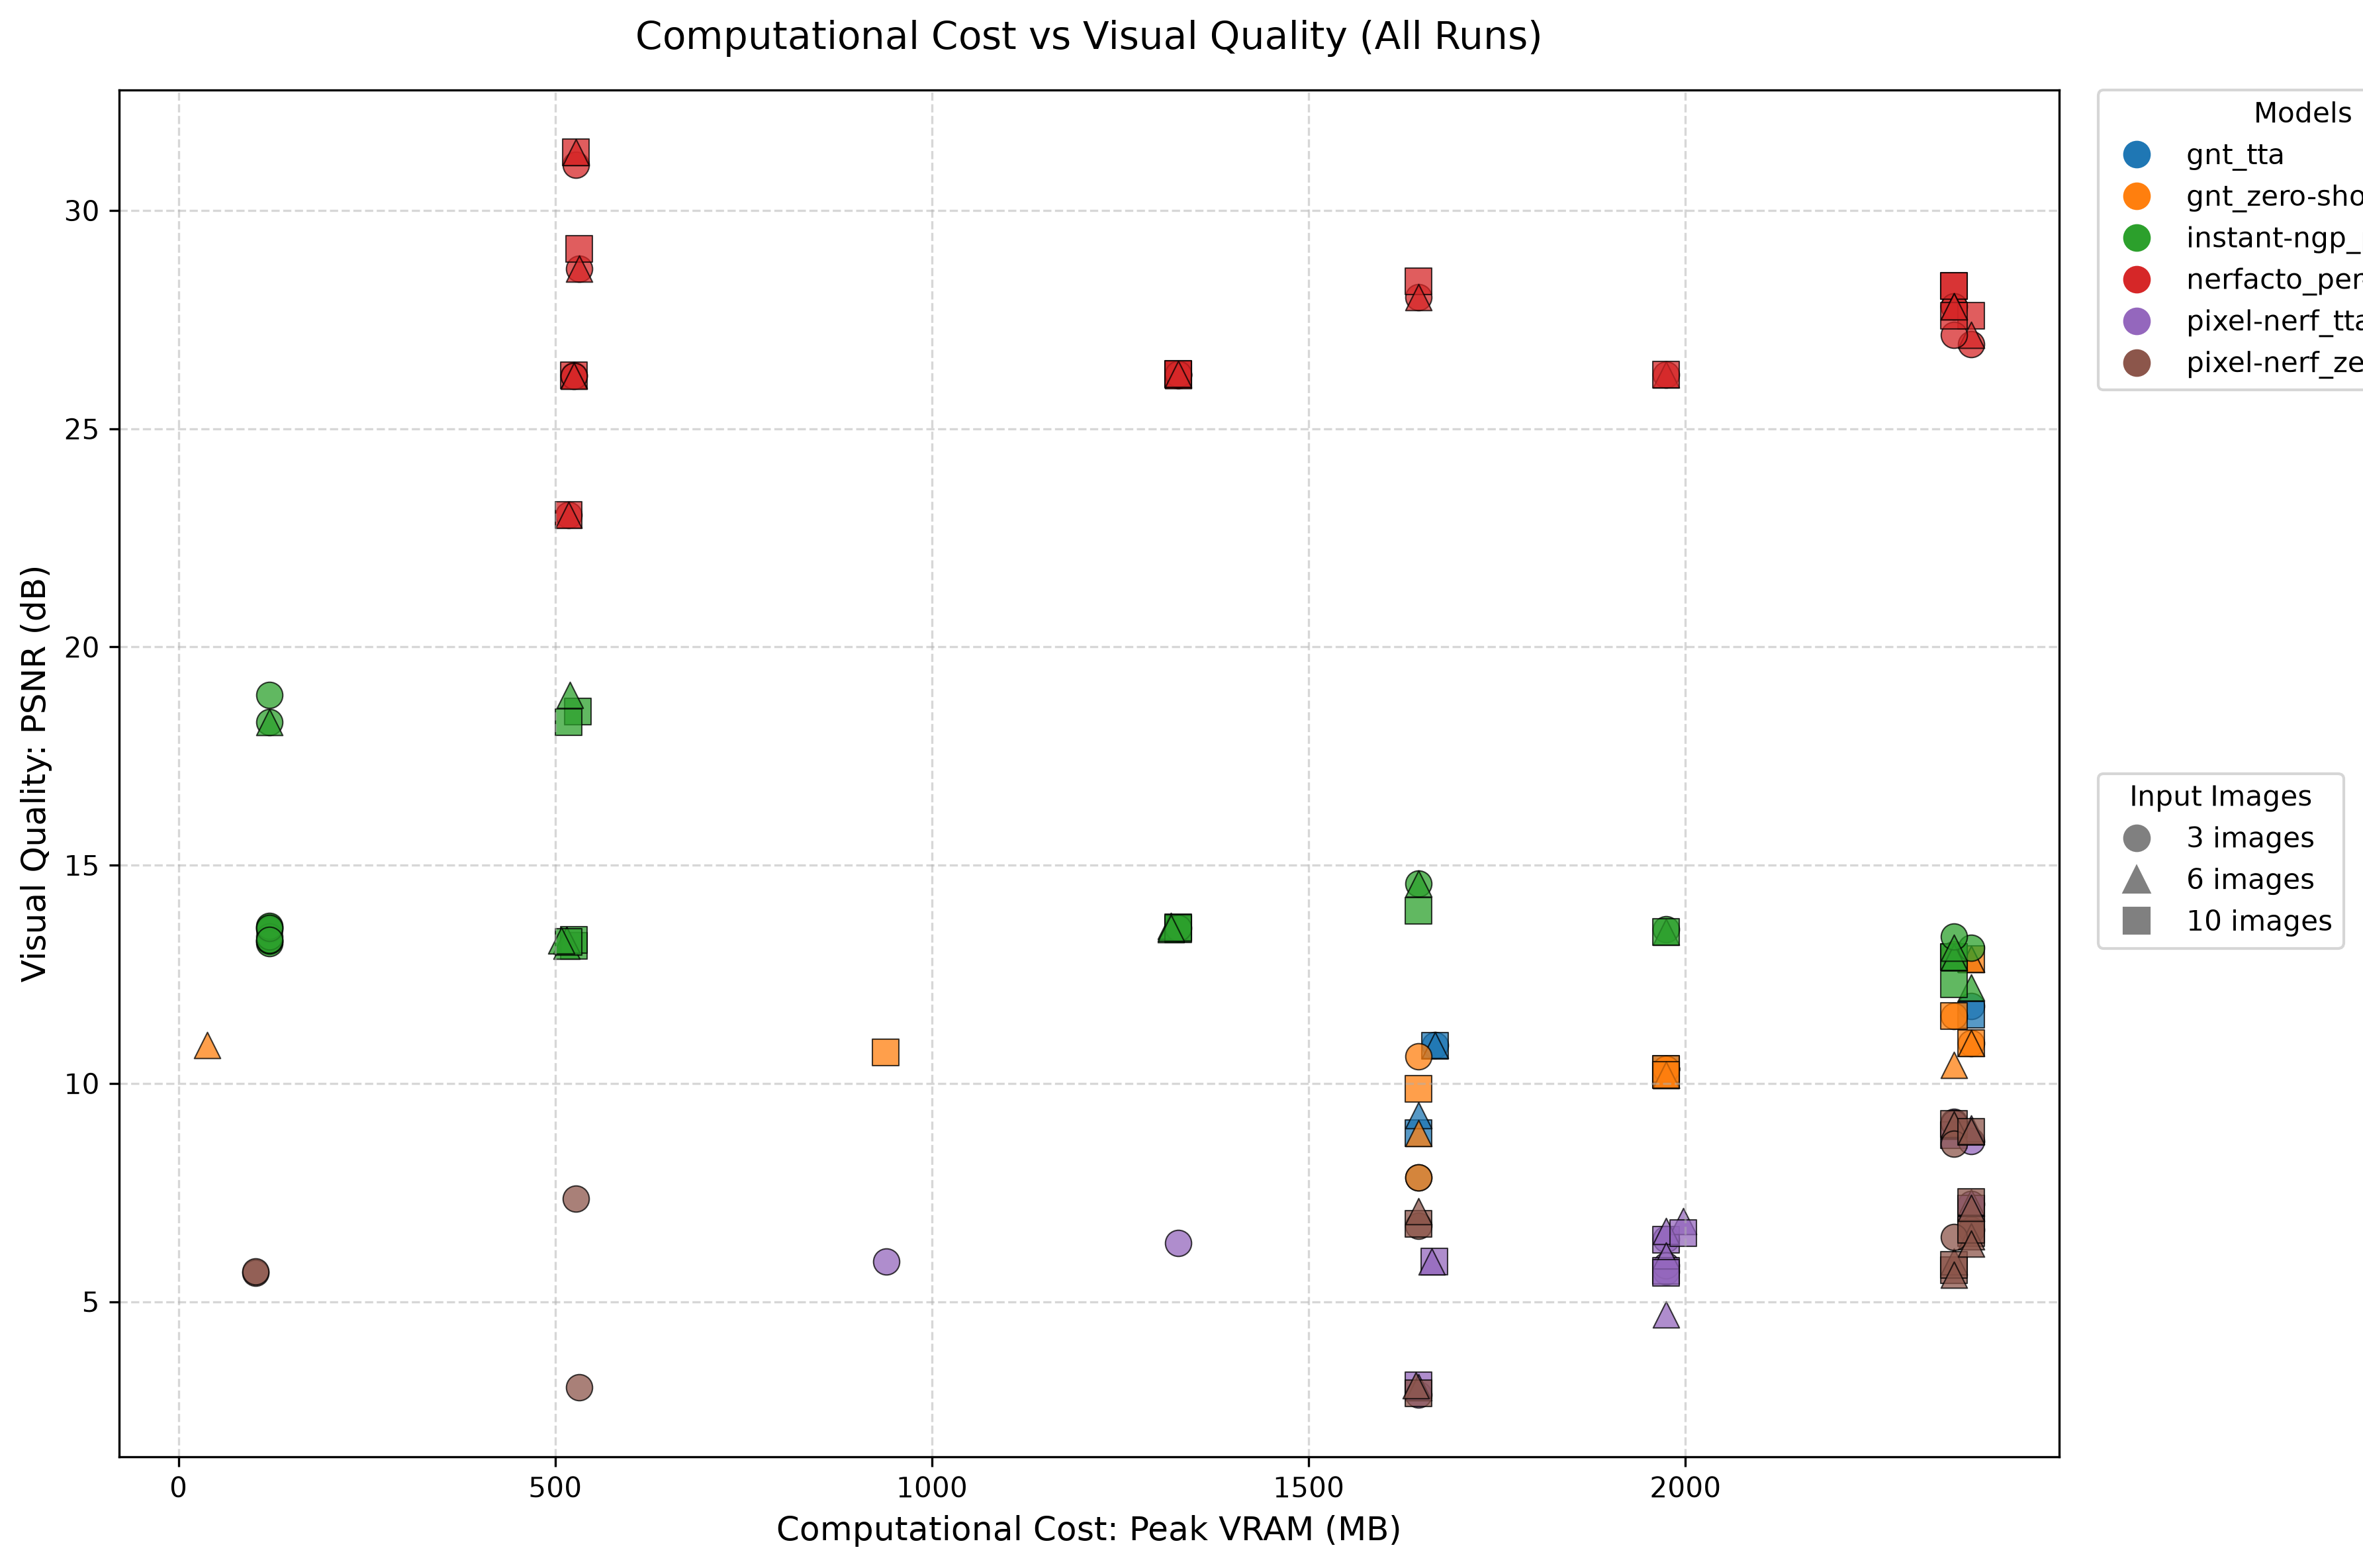
\includegraphics[width=\linewidth]{img/vram_vs_psnr_all_runs_plot.png}
\caption{Trade-off between visual fidelity (PSNR) and computational cost (Peak VRAM) across all evaluated scenes and regimes. The top-left quadrant represents the ideal operational region (high quality, low memory footprint), which is heavily dominated by per-scene hash-based architectures.}
\label{fig:vram_vs_psnr}
\end{figure}
\begin{table*}[!t]
\centering
\caption{Consolidated quantitative results across the LLFF dataset. Metrics represent the global average. Training time reflects the fine-tuning phase for TTA and full convergence for Per-Scene models. VRAM Peak denotes dynamic memory allocation during inference.}
\label{tab:super_results}
\resizebox{\textwidth}{!}{%
\begin{tabular}{llcccccc}
\toprule
\textbf{Paradigm} & \textbf{Model \& Regime} 
  & \textbf{PSNR (dB) $\uparrow$} 
  & \textbf{SSIM $\uparrow$} 
  & \textbf{LPIPS $\downarrow$} 
  & \textbf{Train / TTA Time} 
  & \textbf{Inference (FPS) $\uparrow$} 
  & \textbf{VRAM Peak (GB) $\downarrow$} \\
\midrule
\multirow{4}{*}{\textbf{Generalizable}} 
 & PixelNeRF (Zero-Shot) & 6.62  & 0.093 & 0.814 & $\sim$22 s   & 0.004 & 1.93 \\
 & PixelNeRF (TTA)       & 6.38  & 0.071 & 0.801 & 4 min 23 s   & 0.006 & 1.97 \\
 \cmidrule{2-8}
 & GNT (Zero-Shot)       & 10.73 & 0.300 & 0.760 & $\sim$9 s    & 0.014 & 1.94 \\
 & GNT (TTA)             & 10.42 & 0.336 & 0.724 & 7 min 19 s   & 0.015 & 1.93 \\
\midrule
\multirow{2}{*}{\textbf{Per-Scene}}     
 & Instant-NGP (100\%)   & 14.06 & 0.442 & 0.498 & 31 min 51 s  & 0.199 & \textbf{1.09} \\
 & Nerfacto (100\%)      & \textbf{27.11} & \textbf{0.875} & \textbf{0.171} & 8 min 57 s   & \textbf{0.388} & 1.43 \\
\bottomrule
\end{tabular}%
}
\end{table*}

\subsection{Qualitative Analysis}

The qualitative assessment visually corroborates the quantitative metrics, specifically illustrating the boundaries of each architectural paradigm. For visual clarity, we synthesized novel views matching the exact poses from the test set using perspective projection.

Figure \ref{fig:comparacao_qualitativa} highlights the severe disparities in reconstruction quality on the highly detailed \textit{fern} scene. As visually evident, neither PixelNeRF nor GNT achieved proper convergence. PixelNeRF produced renderings with intense isotropic blurring, a typical artifact indicating the network's failure to accurately localize 2D projected features across extremely sparse views. GNT, on the other hand, demonstrated a complete generalization failure regarding the \textit{in-the-wild} characteristics of the scene. This resulted in a representational visual collapse—heavily distorting the volumetric geometry into noise—which persisted even after the 10-view Test-Time Adaptation (TTA).

Conversely, the per-scene architectures successfully captured the intricate foliage geometry. While Instant-NGP exhibited minor volumetric density fluctuations (floaters) in sparsely covered peripheral regions, Nerfacto produced a highly faithful reconstruction, preserving high-frequency details directly matching the native resolution of the Ground Truth.

\begin{figure}[!t]
    \centering
    % Row 1: Ground Truth (Centered)
    \begin{subfigure}[b]{0.48\linewidth}
        \centering
        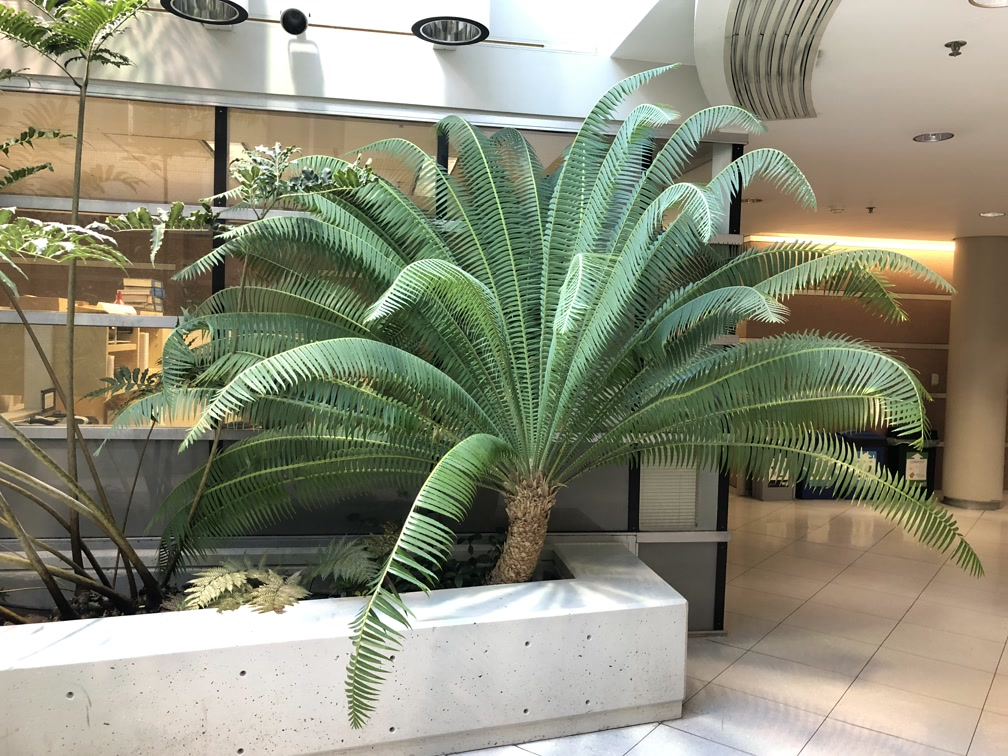
\includegraphics[width=\linewidth]{img/gt.jpg}
        \caption*{Ground Truth}
    \end{subfigure}
    
    \vspace{2mm} % Vertical spacing between rows

    % Row 2: Generalizable Models (The ones that failed)
    \begin{subfigure}[b]{0.48\linewidth}
        \centering
        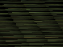
\includegraphics[width=\linewidth]{img/pixel-nerf.png}
        \caption*{PixelNeRF (TTA 10)}
    \end{subfigure}\hfill
    \begin{subfigure}[b]{0.48\linewidth}
        \centering
        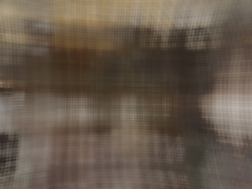
\includegraphics[width=\linewidth]{img/gnt.png}
        \caption*{GNT (TTA 10)}
    \end{subfigure}
    
    \vspace{2mm}
    
    % Row 3: Per-Scene Models (The successful ones)
    \begin{subfigure}[b]{0.48\linewidth}
        \centering
        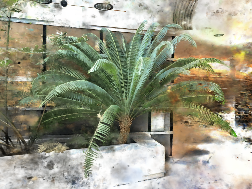
\includegraphics[width=\linewidth]{img/instant-ngp.png}
        \caption*{Instant-NGP (Per-Scene)}
    \end{subfigure}\hfill
    \begin{subfigure}[b]{0.48\linewidth}
        \centering
        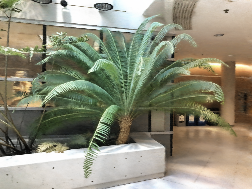
\includegraphics[width=\linewidth]{img/nerfacto.png}
        \caption*{Nerfacto (Per-Scene)}
    \end{subfigure}

    \caption{Qualitative comparison on the \textit{fern} scene. Generalizable architectures (PixelNeRF and GNT) failed to converge under sparse constraints, resulting in severe blurring and visual collapse. In contrast, per-scene optimization models (Instant-NGP and Nerfacto) successfully reconstructed the complex geometry.}
    \label{fig:comparacao_qualitativa}
\end{figure}


\section{Conclusion}

This work developed a methodology for systematically characterizing the trade-offs between computational performance and reconstruction fidelity of Generalizable and Per-Scene NeRF architectures under sparse-view conditions. The experimental results demonstrate that Per-Scene models achieve substantially lower inference latency and VRAM consumption than generalizable models, making them well suited for deployment in resource-constrained environments. However, these benefits rely on dense multi-view supervision, restricting their usage in sparse-view acquisition scenarios, where generalizable architectures remain a practical alternative despite reduced reconstruction fidelity.

Although the proposed strategy provides a standardized and reproducible framework, some limitations should be acknowledged. The restricted hardware configuration of the experimental environment prevented the inclusion of architectures that rely on computationally intensive 3D cost volumes or strong geometric regularization, such as RegNeRF. Furthermore, the experimental validation was conducted on the LLFF dataset, and the adopted sparse-view sampling strategy exploits the sequential ordering of its image indices, which may limit its direct applicability to unordered image collections.

In this context, future work will focus on extending the proposed methodology to unbounded 360-degree datasets and more diverse acquisition scenarios, enabling a broader characterization of these trade-offs. This includes incorporating sparse-view 3D Gaussian Splatting variants \cite{seo2026improvingsparseview3dgsgeneralization,song2025d2gsdepthanddensityguidedgaussian} into the benchmarking protocol, to assess whether their explicit representation offers a more favorable fidelity--efficiency trade-off than the implicit architectures evaluated here. Also, diffusion priors will be investigated as regularization mechanisms during FT to improve reconstruction quality.
\section*{Acknowledgment}
The authors would like to thank State of São Paulo University and the Interdisciplinary Image Processing and Analysis Laboratory for providing the infrastructure necessary to conduct this research.


% references section

% can use a bibliography generated by BibTeX as a .bbl file
% BibTeX documentation can be easily obtained at:
% http://mirror.ctan.org/biblio/bibtex/contrib/doc/
% The IEEEtran BibTeX style support page is at:
% http://www.michaelshell.org/tex/ieeetran/bibtex/
\bibliographystyle{IEEEtran}
% argument is your BibTeX string definitions and bibliography database(s)
\bibliography{example}

\end{document}